\documentclass[10pt]{article}
\usepackage{fullpage,enumitem,amsmath,amssymb,graphicx,listings,tikz,bbm,xcolor,algorithm2e}
\setlength{\parindent}{0pt}

\begin{document}

\begin{center}
{\Large \textbf{Theory Problems: Batch 2}}

\begin{tabular}{rl}
\\
Course: & Coursera Algorithms Specialization \\
Name: & Bryan Yaggi
\end{tabular}
\end{center}

\section*{\normalsize Problem 1}

Prove that the worst-case expected running time of every randomized comparison-based sorting algorithm is $\Omega(n \log ⁡n)$. (Here the worst-case is over inputs, and the expectation is over the random coin flips made by the algorithm.)
\bigskip

In lecture, we showed that any deterministic comparison-based sorting algorithm has a lower bound, $\Omega(n log n)$. First, prove the average-case time is $\Omega(n log n)$. A comparison-based sorting algorithm can be represented as a binary decision tree. See the following example.
\smallskip

Example: Given three elements in a list, $[e_1, e_2, e_3]$.

\begin{center}
  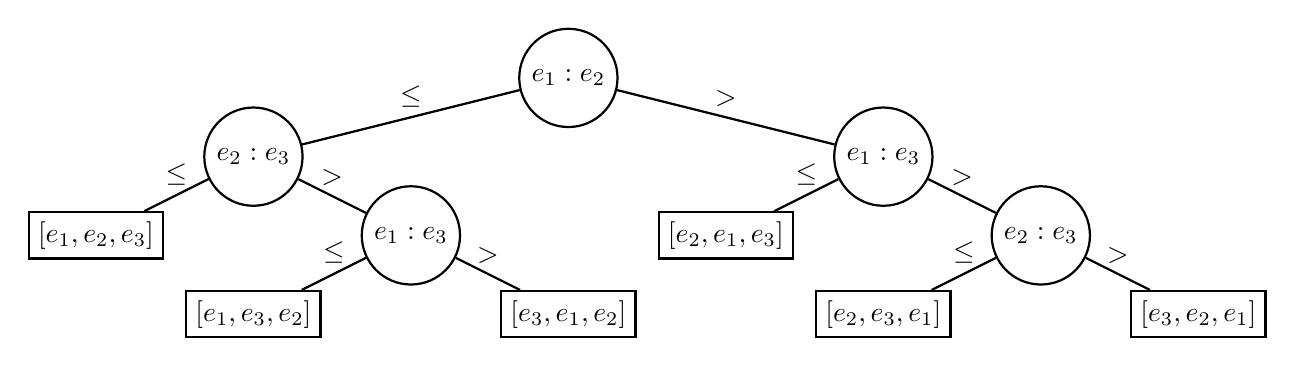
\begin{tikzpicture}
		\begin{scope}[every node/.style={circle,thick,draw}]
    		\node (C11) at (0,0) {$e_1:e_2$};
    		\node (C21) at (-4,-1) {$e_2:e_3$};
    		\node (C22) at (4,-1) {$e_1:e_3$};
    		\node (C31) at (-2,-2) {$e_1:e_3$};
    		\node (C32) at (6,-2) {$e_2:e_3$};
		\end{scope}
		\begin{scope}[every node/.style={thick,draw}]
    		\node (L1) at (-6,-2) {$[e_1, e_2, e_3]$};
    		\node (L3) at (-4,-3) {$[e_1, e_3, e_2]$};
    		\node (L4) at (0,-3) {$[e_3, e_1, e_2]$};
    		\node (L2) at (2,-2) {$[e_2, e_1, e_3]$};
    		\node (L5) at (4,-3) {$[e_2, e_3, e_1]$};
    		\node (L6) at (8,-3) {$[e_3, e_2, e_1]$};
		\end{scope}
		\begin{scope}[every edge/.style={draw=black,thick}]
			\path [-] (C11) edge node [above] {$\leq$} (C21);
			\path [-] (C11) edge node [above] {$>$} (C22);
			\path [-] (C21) edge node [above] {$>$} (C31);
			\path [-] (C22) edge node [above] {$>$} (C32);
			\path [-] (C21) edge node [above] {$\leq$} (L1);
			\path [-] (C22) edge node [above] {$\leq$} (L2);
			\path [-] (C31) edge node [above] {$\leq$} (L3);
			\path [-] (C31) edge node [above] {$>$} (L4);
			\path [-] (C32) edge node [above] {$\leq$} (L5);
			\path [-] (C32) edge node [above] {$>$} (L6);
		\end{scope}
	\end{tikzpicture}
\end{center}

For $n$ elements, there are $n!$ possible permutations, and each permutation has a $\frac{1}{n!}$ probability of being reached. Let $D(T)$ be the external path length of the decision tree, $T$, or the sum of the depths of each leaf in the tree. For any $T$ with $k > 1$ leaves, $D(T) = D(LT) + D(RT) + k$, where $LT$ and $RT$ are the left and right subtrees, respectively. This is true because the leaves of $LT$ and $RT$ are one node shallower than in $T$, and the path to each leaf must go through the root node. Using this observation, the combination of leaves in $LT$ and $RT$ that minimizes $D(T)$ can be found. $D(T) \geq i \log i + (k - i) \log (k - i) + k$ where $i$ is the number of leaves in $LT$.

\begin{align*}
	D(T) &\geq i \log i + (k - i) \log (k - i) + k \\
	\frac{\partial D(T)}{\partial i} &= \log i + 1 - \log(k - i) - 1 = \log \frac{i}{k - i} \\
	\frac{\partial D(T)}{\partial i} &= 0 \iff \frac{i}{k - i} = 1 \implies i = \frac{k}{2}
\end{align*}

This result indicates that $D(T)$ is minimized by a balanced tree. Therefore, $D(T) > k \log k \iff D(T) > n! \log (n!)$. The average-case time, or leaf depth, for sorting $n$ elements is $\log(n!) \implies \Omega(n \log n)$. Now, show the expected running time for random camparison-based sort. A random comparison sort is just a randomly-selected decision tree, $T$ from the set valid decision trees for sorting the input. Let $N$ be the number of valid decision trees.

\begin{align*}
	E(time) &= \sum_{j = 1}^{N} p_j time = \sum_{j = 1}^{N} \frac{1}{N} \Omega(n \log n) \\
	&= \Omega(n \log n)
\end{align*}

\smallskip

See CLRS Problem 8-1 and solution.

\section*{\normalsize Problem 2}

Suppose we modify the deterministic linear-time selection algorithm by grouping the elements into groups of 7, rather than groups of 5. (Use the ``median-of-medians" as the pivot, as before.) Does the algorithm still run in $O(n)$ time? What if we use groups of 3?
\bigskip

In lecture, a 2D grid representation was used to show the problem size reduction of the second recursive call in the DSelect algorithm. In the grid, each column represents a group and subscripts indicate the order for each group. The groups are placed in ascending order by their median elements. When the ``median-of-medians'' is selected, the southwest quadrant of elements is guaranteed to be less than or equal to this element. Likewise, the northeast quadrant of elements is guaranteed to be greater than or equal. The following is an example grid using groups of 5.

$$
\begin{matrix}
	a_5 & b_5 & c_5 & d_5 & e_5 & f_5\\
	a_4 & b_4 & c_4 & d_4 & e_4 & f_4\\
	\textcolor{blue}{a_3} & \textcolor{blue}{b_3} & \textcolor{red}{c_3} & d_3 & e_3 & f_3\\
	\textcolor{blue}{a_2} & \textcolor{blue}{b_2} & \textcolor{blue}{c_2} & d_2 & e_2 & f_2\\
	\textcolor{blue}{a_1} & \textcolor{blue}{b_1} & \textcolor{blue}{c_1} & d_1 & e_1 & f_1 
\end{matrix}
$$

The red element is the ``median-of-medians'' and the blue elements are those guaranteed to be smaller than or equal to it. This means that the number of elements remaining will be $\leq .7n$. The result is $T(n) \leq Cn + T(\frac{n}{5}) + T(\frac{7}{10} n) = O(n)$.
\smallskip

For groups of 7:

$$
\begin{matrix}
	a_7 & b_7 & c_7 & d_7 & e_7 & f_7\\
	a_6 & b_6 & c_6 & d_6 & e_6 & f_6\\
	a_5 & b_5 & c_5 & d_5 & e_5 & f_5\\
	\textcolor{blue}{a_4} & \textcolor{blue}{b_4} & \textcolor{red}{c_4} & d_4 & e_4 & f_4\\
	\textcolor{blue}{a_3} & \textcolor{blue}{b_3} & \textcolor{blue}{c_3} & d_3 & e_3 & f_3\\
	\textcolor{blue}{a_2} & \textcolor{blue}{b_2} & \textcolor{blue}{c_2} & d_2 & e_2 & f_2\\
	\textcolor{blue}{a_1} & \textcolor{blue}{b_1} & \textcolor{blue}{c_1} & d_1 & e_1 & f_1 
\end{matrix}
$$

$T(n) \leq Cn + T(\frac{n}{7}) + T(\frac{5}{7} n) = O(n)$
\smallskip

For groups of 3:

$$
\begin{matrix}
	a_3 & b_3 & c_3 & d_3 & e_3 & f_3\\
	\textcolor{blue}{a_2} & \textcolor{blue}{b_2} & \textcolor{red}{c_2} & d_2 & e_2 & f_2\\
	\textcolor{blue}{a_1} & \textcolor{blue}{b_1} & \textcolor{blue}{c_1} & d_1 & e_1 & f_1 
\end{matrix}
$$

$T(n) \leq Cn + T(\frac{n}{3}) + T(\frac{2}{3} n) > O(n)$

\section*{\normalsize Problem 3}

Given an array of $n$ distinct (but unsorted) elements $x_1, x_2, \dots, x_n$​ with positive weights $w_1, w_2, \dots, w_n$​ such that $\sum_{i=1}^{n} w_i = W$, a weighted median is an element $x_k$​ for which the total weight of all elements with value less than $x_k$​ (i.e., $\sum_{x_i < x_k}$) is at most $W/2$, and also the total weight of elements with value larger than $x_k$​ (i.e., $\sum_{x_i > x_k}$) is at most $W/2$. Observe that there are at most two weighted medians. Show how to compute all weighted medians in $O(n)$ worst-case time.
\bigskip

This can be achieved using an algorithm based on quickselect. The pivot element should be chosen using deterministic selection. Here is pseudocode for the algorithm. $elements$ is a data structure containing the value and weight of each element, $W$ is the sum of weights, $W_{left}$ is the sum of elements to the left of the pivot, and $value(pivot)$ is the value of the pivot element.
\smallskip

\SetKwProg{Fn}{Function}{}{end}
\SetKwFunction{FRecurs}{FindMedians}
\newcommand{\forcond}{$i=0$ \KwTo $n$}

\Fn(){\FRecurs{elements, W, startIndex, endIndex}}{
	\KwIn{\\
	$elements$ is data structure containing value and weight of each element\\
	$W$ is sum of weights\\
	$startIndex$ is start index of elements involved\\
	$endIndex$ is end index of elements involved}
	\KwOut{\\weighted medians}
	\BlankLine
	
	{pick pivot element using deterministic select}\\
	{partition elements based on element values}\\
	\If(\tcc*[h]{$W_{left}$ is sum of element weights to left of pivot}){$W_{left} > \frac{W}{2}$}{\FRecurs{elements, W, startIndex, pivotIndex}\;
		\tcc{recurse on left side of pivot element}
	}
	\If(\tcc*[h]{$value(pivot)$ is the value of the pivot element}){$W_{left} + value(pivot) \leq \frac{W}{2}$}{\FRecurs{elements, W, pivotIndex+1, endIndex}\;
		\tcc{recurse on right side of pivot element}
	}
	{left weighted median found}\\
	\If(\tcc*[h]{$value(pivot)$ is the value of the pivot element}){$W - W_{left} - value(pivot) > \frac{W}{2}$}{right weighted median is smallest element of those right of pivot\;
	}
}

\section*{\normalsize Problem 4}

We showed in an optional video lecture that every undirected graph has only polynomially (in the number $n$ of vertices) different minimum cuts. Is this also true for directed graphs? Prove it or give a counterexample.
\bigskip

Answer...

\section*{\normalsize Problem 5}

For a parameter $\alpha \geq 1$, an $\alpha$-minimum cut is one for which the number of crossing edges is at most $\alpha$ times that of a minimum cut. How many $\alpha$-minimum cuts can an undirected graph have, as a function of $\alpha$ and the number $n$ of vertices? Prove the best upper bound that you can.
\bigskip

Answer...

\end{document}
